\begin{figure}[t]
    \centering
    \resizebox{\textwidth}{!}{%
    \begin{tikzpicture}[font={\footnotesize},trap/.style={trapezium, rotate=-90,trapezium angle=75},]
        %% CNN branch
        \node(input) at (-5.5, 0) {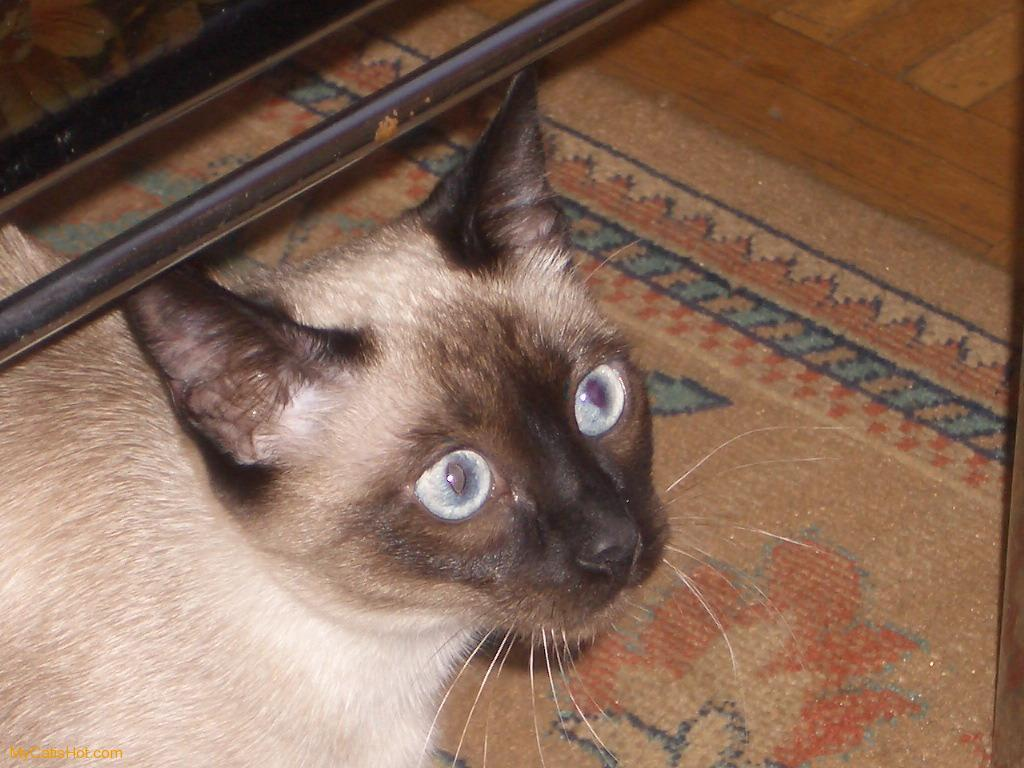
\includegraphics[width=.1\textwidth]{fig/castream/images/input.jpg}};
        \node[above] at (input.north) {Input image $\vx$};
        \node[draw, trap] (res0) at (-3.5,0) {\rotatebox{90}{\parbox{1.0cm}{\centering{Res-0}}}};
        \node[draw, trap] (res1) at (-1.5,0) {\rotatebox{90}{\parbox{1.0cm}{\centering{Res-1}}}};
        \node[draw, trap] (res2) at (0.5,0) {\rotatebox{90}{\parbox{1.0cm}{\centering{Res-2}}}};
        \node[draw, trap] (res3) at (2.5,0) {\rotatebox{90}{\parbox{1.0cm}{\centering{Res-3}}}};
        \node[draw, trap] (res4) at (4.5,0) {\rotatebox{90}{\parbox{1.0cm}{\centering{Res-4}}}};
        \node[](empt1) at (6.75, 0){};
        \node[draw, rotate=90, align=center] (class) at (7.5,0) {Classifier};
        \node(logit) at (8.25, 0) {$\vy$};
        %%% CLS stream
        \node[](clsin) at (-4, -1.5) {{$\vq_0$}};
        \node[draw](CA0) at (-2.5, -1.5) {{CA-0}};
        \node[draw](CA1) at (-0.5, -1.5) {{CA-1}};
        \node[draw](CA2) at (1.5, -1.5)  {{CA-2}};
        \node[draw](CA3) at (3.5, -1.5)  {{CA-3}};
        \node[draw](CA4) at (5.5, -1.5)  {{CA-4}};
    
        %% CNN backbone
        \node(empt0) at (-4.65, 0) {};
        \draw[->] (empt0.center) -- node {} (res0);
        \draw[->] (res0) -- node[above] {$F_0$} (res1);
        \draw[->] (res1) -- node[above] {$F_1$} (res2);
        \draw[->] (res2) -- node[above] {$F_2$} (res3);
        \draw[->] (res3) -- node[above] {$F_3$} (res4);
        \draw[->, blue, dashed] (res4) -- node {\blue{\normalsize//}} (class);
        \node[](GAP) at (6.25,0.25) {\blue{$\gap$}};
        \draw[->] (class) -- node {} (logit);
        %% CLS Stream
        \draw[->] (clsin) -- node {} (CA0);
        \draw[dashed, ->] (res0.north) -|node {} (CA0);
        \draw[->] (CA0) -- node[above] {$\vq_1$} (CA1);
        \draw[dashed, ->] (res1.north) -|node {} (CA1);
        \draw[->] (CA1) -- node[above] {$\vq_2$} (CA2);
        \draw[dashed, ->] (res2.north) -|node {} (CA2);
        \draw[->] (CA2) -- node[above] {$\vq_3$} (CA3);
        \draw[dashed, ->] (res3.north) -|node {} (CA3);
        \draw[->] (CA3) -- node[above] {$\vq_4$} (CA4);
        \draw[dashed, ->] (res4.north) -|node[above] {$F_4$} (CA4);
        \draw[-] (CA4.east) -| node[right] {$\vq_5$} (empt1.center);
        \draw[->] (empt1.center) -- node {} (class);
    \end{tikzpicture}
    }
    \vspace{3pt}
    \caption{\emph{\OURS (\Ours) applied to ResNet-based architectures.} Given a network $f$, we 
             replace global average pooling (\gap) by a learned, attention-based pooling mechanism 
             implemented as a stream in parallel to $f$. The feature tensor $F_\ell \in 
             \real^{p_\ell \times d_\ell}$ (\emph{key}) obtained by stage Res-$\ell$ of $f$ 
             interacts with a \cls token (\emph{query}) embedding $\vq_\ell \in \real^{d_\ell}$ in 
             block CA-$\ell$, which contains cross attention~\eq{CA} followed by a linear 
             projection~\eq{qk-layer} to adapt to the dimension of $F_{\ell+1}$. Here, $p_\ell$ is 
             the number of patches (spatial resolution) and $d_\ell$ the embedding dimension. The 
             query is initialized by a learnable parameter $\vq_0 \in \real^{d_0}$, while the output 
             $\vq_5$ of the last cross attention block is used as a global image representation into 
             the classifier.}
    \label{fig:fig_method}
    \end{figure}
    